\documentclass[../analysis1.tex]{subfiles}

\begin{document}


\chapter{Limits and Continuity}

In this chapter, we move on from thinking about \textit{sequences}, which are functions $\N\to\R$, and we start to build some theory for functions $\R\to\R$, in particular what constitutes a ``\textit{nice}'' function.\par
What motivates this chapter is that a ``\textit{nice}'' function should be able to drawn without taking our pen off the paper, because we expect nice properties of such functions; this is intuition is a property called the ``\textit{Intermediate Value Property}'', and does indeed hold for \textit{continuous} functions (but is not exclusive to continuous functions).\par
However, the above discussion is by no means a definition. We will define what we mean by \textit{continuity} of a function $f:\R\to\R$ once we understand what a \textit{limit} of a function is. In particular, since we are working with functions whose domain is $\R$ now, the notion of \textit{limit} can be made meaningful without sending $x\to\infty$ (i.e. we can define the limit of a function $f(x)$, say, as $x\to a$ where $a\in \R$ is some real number).


\section{Limits of Functions}
We wish to adapt the definition of limit for functions $\R\to\R$. First, we make the definition for limits as $|x|\to\infty$, which are analogous to the definition of a limit for sequences (but of course, rather than only being able to send $n$ to positive infinity like in sequences, there is another direction, the negative numbers, so we can also define limits as $x\to-\infty$ as well).

\begin{definition}
    \begin{shaded*}
        Let $f:\R\to\R$ be a function, and let $L\in\R$.
        \begin{enumerate}
            \item[1.] We say that $f(x)$ tends to $L$ as $x\to\infty$ if
            \[\forall \varepsilon>0,\,\exists R\in\R,\, \forall x\ge R,\, |f(x)-L|<\varepsilon.\] 
            \item[2.] We say that $f(x)$ tends to $L$ as $x\to-\infty$ if
            \[\forall \varepsilon>0,\,\exists R\in\R,\, \forall x\le R,\, |f(x)-L|<\varepsilon.\] 
        \end{enumerate}
    \end{shaded*}
\end{definition}




\begin{definition}
    \begin{shaded*}
        Let $f:\R\to\R$ be a function.
        \begin{enumerate}
            \item[1.] We say that $f(x)$ tends to $\infty$ as $x\to\infty$ if
            \[\forall M>0,\,\exists R\in\R,\, \forall x\ge R,\, f(x)>M.\] 
            \item[2.] We say that $f(x)$ tends to $\infty$ as $x\to-\infty$ if
            \[\forall M>0,\,\exists R\in\R,\, \forall x\le R,\, f(x)>M.\] 
        \end{enumerate}
    \end{shaded*}
\end{definition}
There is an obvious variation of the above definitions for the definitions of $\lim_{x\to\infty}f(x)=-\infty$ and $\lim_{x\to-\infty}f(x)=-\infty$.\par
To define ``$\lim_{x\to a}f(x)=L$'', we need to be precise about what ``for $x$ close enough to a'' actually means. Also, it is going to matter whether we approach a from the side $x>a$ or from the side $x<a$, so writing $\lim_{x\to a}f(x)=L$ may not always make sense.

\begin{definition}
    \begin{shaded*}
        Let $a\in\R$ and let $f:(a,\infty)\to\R$ be a function. We say that $f(x)$ tends to $L\in\R$ as $x\to a^+$ if
        \[\forall\varepsilon>0,\,\exists\delta>0,\,\forall x\in(a,\infty),\, x\in(a,a+\delta)\implies |f(x)-L|<\varepsilon.\]
    \end{shaded*}
\end{definition}
Above, we formalised ``for $x>a$ sufficiently close to $a$'' as ``$x\in (a,a+\delta)$ for some $\delta>0$''.

\begin{definition}
    \begin{shaded*}
        Let $a\in\R$ and let $f:(b,a)\to\R$ be a function for some $b<a$. We say that $f(x)$ tends to $L\in\R$ as $x\to a^-$ if
        \[\forall\varepsilon>0,\,\exists\delta>0,\,\forall x\in(b,a),\, x\in(a-\delta,a)\implies |f(x)-L|<\varepsilon.\] 
    \end{shaded*}
\end{definition}


\begin{remark}
    Limits are entirely about the behaviour of $f$ \textit{near} $a$, not \textit{at} $a$. The value $f(a)$ does not even need to be defined. If $\lim_{x\to a} f(x) = L$ exists but $f(a)$ is undefined or doesn't equal $L$, we can define a ``continuous extension'' $\tilde{f}$ where $\tilde{f}(x) = f(x)$ for $x \neq a$ and $\tilde{f}(a) = L$. This is a useful trick for when we want to apply some stronger theorems which only apply to, say, continuous functions.
\end{remark}

\begin{center}
\begin{minipage}{1.0\textwidth}
\centering
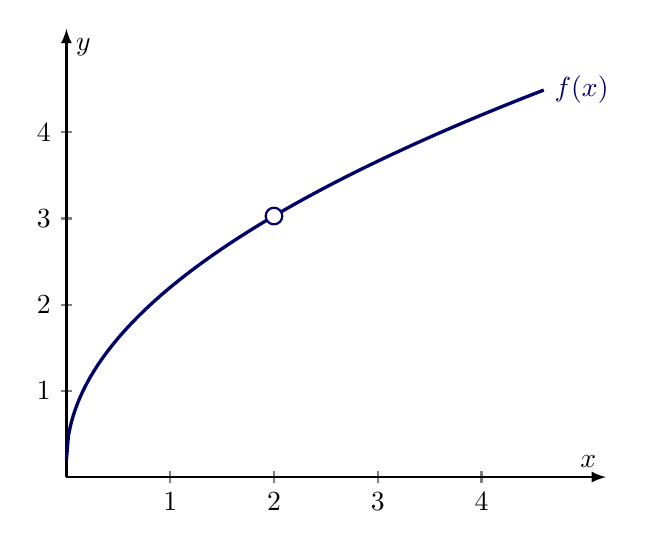
\begin{tikzpicture}
    \begin{axis}[
        axis lines = middle,
        xmin=0, xmax=5.2,
        ymin=0, ymax=5.2,
        %grid=major,
        xlabel={$x$},
        ylabel={$y$},
        xtick={1,2,3,4},
        ytick={1,2,3,4},
        tick style={thick},
        % Ensure the plot area is clean
        axis line style={-latex, thick},
        clip=false
    ]
        % Function before the hole (0 to 1.95)
        \addplot [
            domain=0:1.93, 
            samples=100, 
            very thick, 
            blue!40!black
        ] {sqrt(x)*2 + 0.2};
        
        % Function after the hole (2.05 to 4.6)
        \addplot [
            domain=2.07:4.6, 
            samples=100, 
            very thick, 
            blue!40!black
        ] {sqrt(x)*2 + 0.2} node[right] {$f(x)$};
        
        % The Removable Discontinuity (The Hole)
        % Coordinates calculated from the function: f(2) = sqrt(2)*2 + 0.2 ≈ 3.03
        \addplot [
            only marks, 
            mark=o, 
            mark size=3pt, 
            thick, 
            blue!40!black, 
            fill=white
        ] coordinates {(2, 3.028)};
        
    \end{axis}
\end{tikzpicture}
\end{minipage}
\end{center}

For example, in the picture above, the function $f(x)$ has $\allowbreak\lim_{x\to 2^-} f(x)=\lim_{x\to 2^+} f(x)=3$, but is not defined at $x=2$. If we defined $f(2)=3$, then $f$ would be a continuous function.


\begin{lemma}
    \begin{shaded*}
        Suppose $f:(a,b)\to\R$ is a function, and we have \[\lim_{x\to a^+}f(x)=L_1\quad\text{and}\quad\lim_{x\to a^+}f(x)=L_2.\]
        Then $L_1=L_2$.
    \end{shaded*}
\end{lemma}
\begin{proof}
    Let $\varepsilon>0$ be arbitrary. Since $\lim_{x\to a^+}f(x)=L_1$, we can let $\delta_1>0$ be such that for any $x\in (a,a+\delta_1)$, $|f(x)-L_1|<\frac{\varepsilon}{2}$.
    Similarly, since $\lim_{x\to a^+}f(x)=L_2$, we can let $\delta_2>0$ be such that for any $x\in(a,a+\delta_2)$, $|f(x)-L_2|<\frac{\varepsilon}{2}$. Let $\delta=\min\{\delta_1,\delta_2\}$ and pick $x\in (a,a+\delta)$. By the triangle inequality we have
    \[|L_1-L_2|=|L_1-f(x)+f(x)-L_2|\le |f(x)-L_1|+|f(x)-L_2|=\frac{\varepsilon}{2}+\frac{\varepsilon}{2}=\varepsilon,\]
    so since $\varepsilon>0$ was arbitrary, it follows that $L_1=L_2$.\qedhere
\end{proof}
This lemma holds if we replace $x\to a^+$ with $x\to a^-$ and the proof is identical. Note that the above fact does not say that we must have $\lim_{x\to a^-} f(x)=\lim_{x\to a^+}$, even if both exist.\par
Now we will define a two-sided limit; note that this requires both the left and right limits to exist and $\lim_{x\to a^-} f(x)=\lim_{x\to a^+}$. The function must also be defined on an interval of the form $(b,c)\setminus\{a\}$ for some $b<a<c$ (notice again that $f(a)$ need not be defined for this definition to make sense):
\begin{definition}
    \begin{shaded*}
        Let $a\in\R$ and let $f:(b,c)\setminus\{a\}:\to\R$ be a function for some $b<a<c$. We say that $f(x)$ tends to $L\in\R$ as $x\to a$ if \[\lim_{x\to a^-} f(x)=L\quad\text{and}\quad\lim_{x\to a^+}f(x)=L.\]
        In other words, $\lim_{x\to a}f(x)=L$ if
        \[\forall\varepsilon>0,\,\exists\delta>0,\,\forall x\in(b,c)\setminus\{a\},\, 0<|x-a|<\delta\implies |f(x)-L|<\varepsilon.\]
    \end{shaded*}
\end{definition}

\begin{definition}
    \begin{shaded*}
        Let $I\subset\R$. We say that $I$ is an \textit{open interval} if it is a set of the form:
        \begin{itemize}
            \item an interval $(a,b)$ for some $a<b$ in $\R$,
            \item an interval $(-\infty,b)$,
            \item an interval $(a,\infty)$,
            \item $I=\R$.
        \end{itemize}
    \end{shaded*}
\end{definition}

\begin{theorem}[Algebra of Limits]
\label{thm:altfunctions}
    \begin{shaded*}
        Let $I\subset\R$ be an open interval, and let $a\in I$. If $\lim_{x \to a} f(x) = L$ and $\lim_{x \to a} g(x) = M$, then:
        \begin{enumerate}
            \item[1.] $\lim_{x \to a} (f(x) + g(x)) = L + M$;
            \item[2.] $\lim_{x \to a} (f(x)g(x)) = LM$;
            \item[3.] $\lim_{x \to a} \frac{1}{f(x)} = \frac{1}{L}$ (provided $L \neq 0$ and $f(x) \neq 0$ near $a$, except possibly at $a$).
        \end{enumerate}
    \end{shaded*}
\end{theorem}
\begin{proof}
    Exercise (compare with the proofs for the Algebra of Limits for sequences).\qedhere
\end{proof}


\begin{remark}
    Let $I \subset \R$ be an interval, and let $a \in I$. When we say a property holds ``near $a$'', we mean there exists some $\delta > 0$ such that the property holds for all $x \in (a-\delta, a+\delta) \cap I$. 
    
    When we append the phrase ``except possibly at $a$'', we restrict $x$ to the punctured neighborhood $0 < |x-a| < \delta$. Therefore, when talking about limits, we can concisely discuss properties of functions that only need to hold \textit{locally}.
    For example, a common requirement for theorems which involve limits of functions like $\frac{1}{f(x)}$ is that $f(x) \neq 0$ near $a$, except possibly at $a$.
\end{remark}


\section{Continuity}

\begin{definition}[Continuity at a point]
    \begin{shaded*}
        Let $I\subset\R$ be an open interval, and let $f:I\to\R$ be a function. We say that $f$ is \textit{continuous} at $a\in I$ if
        \[\lim_{x\to a}f(x)=f(a).\]
        Equivalently, $f$ is continuous at $a\in I$ if
        \[\forall\varepsilon>0,\,\exists\delta>0,\,\forall x\in I,\, |x-a|<\delta\implies |f(x)-f(a)|<\varepsilon.\]
    \end{shaded*}
\end{definition}
\begin{remark}
    Note that we do not need to specify that $|x-a|>0$ since we are assuming $f$ is defined at $a$ now, and if $|x-a|=0$ then $x=a$ and the inequality $|f(a)-f(a)|<\varepsilon$ is trivially satisfied for any $\varepsilon>0$. 
\end{remark}
\begin{exercise*}
    Negate the above string of quantifiers to get a definition for \textit{discontinuity} at a point $a\in I$.
\end{exercise*}

\begin{definition}
    \begin{shaded*}
        Let $I\subset\R$ be an open interval. We say that $f:I\to\R$ is \textit{continuous everywhere}, or \textit{continuous}, if $f$ is continuous at $a$ for all $a\in I$.
    \end{shaded*}
\end{definition}

\begin{example}
\label{ex:basiccontinuityexamples}
    \begin{enumerate}
        \item[1.] Constant functions are continuous everywhere. Indeed, fix $\lambda\in\R$, and define $f:\R\to\R$ by $f(x)=\lambda$ for all $x\in\R$. Let $\varepsilon>0$ and $a\in\R$ be arbitrary. Choose $\delta=1$, and let $x\in\R$ satisfy $|x-a|<\delta$. Then we have \[|f(x)-f(a)|=|\lambda-\lambda|=0<\varepsilon,\]
        so $f$ is continuous everywhere.
        \item[2.] The function $f:\R\to\R$ defined by $f(x)=x$ is continuous everywhere. Indeed, let $\varepsilon>0$ and $a\in\R$ be arbitrary. Choose $\delta=\varepsilon$ and let $x\in\R$ be such that $|x-a|<\delta$. Then we have \[|f(x)-f(a)|=|x-a|<\delta=\varepsilon,\]
        so $f$ is continuous everywhere.
        \item[3.] The function $f:\R\to\R$ defined by \[f(x)=\begin{cases}1,& x\ge 0\\ 0,& x<0\end{cases}\]
        is continuous everywhere except at $a=0$. First we show discontinuity at $a=0$. Pick $\varepsilon=\frac{1}{2}$, and let $\delta>0$ be arbitrary. We know that $f(a)=1$, so we let $x=-\frac{\delta}{2}\in(-\delta,\delta)$. Then we have \[|f(x)-f(0)|=|0-1|=1>\frac{1}{2}=\varepsilon,\]
        so $f$ is discontinuous at $a=0$\par
        Now, let $\varepsilon>0$ and $c\ne 0$ be arbitrary. Choose $\delta=\frac{|c|}{2}$, and let $x\in\R$ be such that $|x-c|<\delta$. Then in particular, \[\frac{|c|}{2}<|x|<\frac{3|c|}{2},\]
        so if $x<0$, then $f(x)=f(c)=0$, and if $x>0$, then $f(x)=f(c)=1$, so in either case $|f(x)-f(c)|=0<\varepsilon$, so $f$ is continuous at $c$ for every $c\ne 0$.
    \end{enumerate}
\end{example}

\subsection{Properties of Continuous Functions}

\begin{theorem}[Algebra for Continuous Functions]
\label{thm:algebracontinuity}
    \begin{shaded*}
        Let $I\subset\R$ be an open interval and let $f,g:I\to\R$ be continuous. Then
        \begin{enumerate}
            \item[1.] $f+g:I\to\R$ is continuous;
            \item[2.] $fg:I\to\R$ is continuous;
            \item[3.] If $f(x)\ne 0$ for all $x\in I$ then the function $\frac{1}{f}:I\to\R$ is continuous. 
        \end{enumerate}
    \end{shaded*}
\end{theorem}
\begin{proof}
    All items follow from the Algebra of Limits for functions (Theorem \ref{thm:altfunctions}).\qedhere
\end{proof}


\begin{example}
\label{ex:polycontinuity}
    In Example \ref{ex:basiccontinuityexamples}, we showed that the identity function on $\R$ is continuous, and constant functions on $\R$ are continuous. Therefore, by induction, for every $n\in\N$, $x\mapsto a_nx^n$ where $a_n\in\R$ is a constant is continuous on $\R$ using item 2 in the Algebra for Continuous functions (Theorem \ref{thm:algebracontinuity}). Using item 1 in the Algebra for Continuous Functions inductively, we deduce that \textit{polynomials} are continuous, i.e. functions $P:\R\to\R$ of the form
    \[P(x)=a_0+a_1x+\cdots+a_{n-1}x^{n-1}+a_nx^n,\]
    where $a_0,\dots,a_n\in\R$ with $a_n\ne 0$ are constants, are continuous.\par
    Furthermore, using this fact, by combining items 2 and 3 in the Algebra for Continuous functions we also deduce that functions of the form \[R:I\to\R,\quad x\mapsto\frac{P(x)}{Q(x)},\]
    where $P,Q$ are polynomials and $I\subset\R$ is an open interval on which $Q$ never vanishes, are continuous. Such a function is called a \textit{rational function}.
\end{example}

\begin{theorem}
\label{thm:compcontinuity}
    \begin{shaded*}
        Let $I\subset\R$ be an open interval, and let $f:I\to\R$ be continuous. Let $J\subset\R$ be an open interval such that $J\supset f(I)$, and let $g:J\to \R$ be continuous. Then
        \[g\circ f:I\to\R\] is continuous.
    \end{shaded*}
\end{theorem}
\begin{proof}
    Let $\varepsilon>0$ and $a\in I$ be arbitrary. Since $\allowbreak g:J\to\R$ is continuous at $f(a)\in J$, there exists $\delta>0$ such that for all $y\in J$, if $|y-f(a)|<\delta$ then $|g(y)-g(f(a))|<\varepsilon$. Since $f:I\to \R$ is continuous at $a\in I$, there exists $\delta'>0$ such that for all $x\in I$, if $|x-a|<\delta'$ then $|f(x)-f(a)|<\delta$. Therefore, we have, for $x\in I$ with $|x-a|<\delta'$, $|f(x)-f(a)|<\delta$, so it follows that (with $y=f(x)$),
    \[|g(f(x))-g(f(a))|<\varepsilon,\]
    so $g\circ f$ is continuous.\qedhere
\end{proof}

\begin{example}
    Using the above Theorem \ref{thm:compcontinuity} and Example \ref{ex:polycontinuity} (where we deduced the continuity of polynomials and rational functions on $\R$), we can deduce the continuity of a large class of functions without having to use the $\varepsilon$-$\delta$ definition. For example, if for the moment we assume the continuity of the functions $\sin$, $\cos$ and $\exp$ (which we will show in later chapters), we can deduce that
    \[x\mapsto \sin\left(\frac{x}{x^2+1}\right),\quad x\mapsto \sum_{k=1}^n \frac{1}{k\pi}\cos(kx),\quad x\mapsto\exp\left(-x^2\right)\]
    are all continuous on $\R$.
\end{example}


\subsection{Sequential Continuity}

We can translate problems about continuity back into the familiar world of sequences with the following concept (which is a bit more general than the $\varepsilon$-$\delta$ definition):
\begin{definition}[Sequential Continuity]
    \begin{shaded*}
        Let $I\subset\R$ be an open interval. A function $f:I\to\R$ is \textit{sequentially continuous} at $a\in I$ if for any sequence $(x_n)$ contained in $I$ with $\lim_{n\to\infty}x_n=a$, we have $\lim_{n\to\infty}f(x_n)=f(a)$.
    \end{shaded*}
\end{definition}
\begin{remark}
    We say that a function $f:I\to\R$, where $I\subset\R$ is an open interval, is \textit{sequentially continuous} if it is sequentially continuous at every $a\in I$.
\end{remark}
In $\R$ (and, in fact, in any metric space) the concepts of sequential continuity and $\varepsilon$-$\delta$ continuity are logically equivalent:
\begin{theorem}[Sequential Characterisation of Continuity]
\label{thm:sequentialcontinuity}
    \begin{shaded*}
        Let $I\subset\R$ be an open interval and let $f:I\to\R$ be a function. Then $f$ is continuous at $a\in I$ if and only if $f$ is sequentially continuous at $a\in I$.
    \end{shaded*}
\end{theorem}
\begin{proof}
    Suppose $f$ is continuous at $a\in I$, and let $\varepsilon>0$ be arbitrary. By definition, we can choose $\delta>0$ such that for all $x\in I$ such that $|x-a|<\delta$, $|f(x)-f(a)|<\varepsilon$. Since $x_n\to a$ as $n\to\infty$, we can let $N\in\N$ be such that for all $n\ge N$, $|x_n-a|<\delta$. Therefore, $|f(x_n)-f(a)|<\varepsilon$ for $n\ge N$, so $f(x_n)\to f(a)$ as $n\to\infty$.\par
    Conversely, suppose $f$ is sequentially continuous at $a\in I$, and suppose for contradiction that $f$ is not continuous at $a\in I$. Therefore, there exists some $\varepsilon_0>0$ such that for all $\delta>0$, there exists $x\in I$ such that $|x-a|<\delta$ and $|f(x)-f(a)|\ge \varepsilon_0$. In particular, for $n\in\N$ we can let $\delta_n\coloneqq\frac{1}{n}$, and by definition we can pick $x_n\in I$ with $|x_n-a|<\delta_n$ such that $|f(x_n)-f(a)|\ge \varepsilon_0$; by induction this defines a sequence $(x_n)$ contained in $I$. However, $x_n\to a$ as $n\to\infty$, but $f(x_n)\not\to f(a)$ as $n\to\infty$, which contradicts sequential continuity of $f$ at $a\in I$.\qedhere
\end{proof}
\begin{remark}
    To prove discontinuity of $f:I\to \R$ at $a\in I$ where $I\subset\R$ is an open interval, it therefore suffices to find \textit{one} sequence $(x_n)$ in $I$ such that $x_n\to a$ but $f(x_n)\not\to f(a)$.
\end{remark}

\begin{example}
    The function $f:\R\to\R$ defined by \[f(x)=\begin{cases}\sin\left(\frac{1}{x}\right),& x\ne 0\\ 0, & x=0\end{cases}\]is not continuous at $0$.
    \begin{center}
    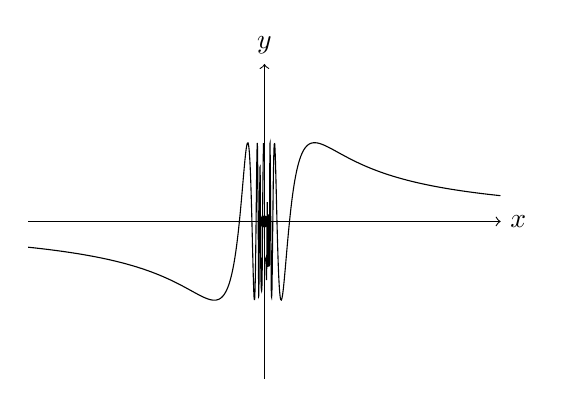
\begin{tikzpicture}
        \draw [->] (-3, 0) -- (3, 0) node [right] {$x$};
        \draw [->] (0, -2) -- (0, 2) node [above] {$y$};
        \draw [domain=-3:-0.01, samples=350, smooth] plot (\x, {sin(deg(1/(\x)))});
        \draw [domain=0.01:3, samples=350, smooth] plot (\x, {sin(deg(1/(\x)))});
        % Origin 
        \filldraw (0,0) circle (2pt);
    \end{tikzpicture}
    \end{center}
    The idea is that for any $\delta>0$, the function $f$ oscillates infinitely many times on the interval $(0,\delta)$, so in particular we can take a sequence converging to zero where the function is constantly 1, which is not equal to $f(0)=0$.\par
    Let $x_n=\frac{1}{2\pi n+\frac{\pi}{2}}$. Then $x_n\to 0$, but $f(x_n)=\sin\left(2\pi n+\frac{\pi}{2}\right)=1$ for all $n\in\N$, so $f(x_n)\to 1\neq 0 = f(0)$, so $f$ is discontinuous at 0.
\end{example}

\begin{exercise*}
    Show that the function $\chi_\Q:\R\to\R$ defined by \[\chi_\Q(x)\coloneqq\begin{cases}1,& x\in\Q\\ 0,& x\notin \Q\end{cases}\]
    is discontinuous everywhere. \textit{(Hint: use the sequential definition of density.)}
\end{exercise*}

\subsection{The Extreme Value Theorem}
We now define continuity on closed and bounded intervals (i.e. intervals of the form $[b,c]$ for some $b<c$ in $\R$. Before, we were only working with open intervals. The definition for continuity on such an interval is a natural extension of continuity on open intervals:
\begin{definition}
    \begin{shaded*}
        Let $K=[b,c]$ be a closed and bounded interval for some $b<c$ in $\R$ and let $f:K\to\R$ be a function. We say that $f$ is \textit{continuous} on $K$ (or just \textit{continuous}) if $f$ is continuous on $(b,c)$ and also \[\lim_{x\to b^+}f(x)=f(b),\quad \lim_{x\to c^-}f(x)=f(c). \]
    \end{shaded*}
\end{definition}

\begin{lemma}
    \begin{shaded*}
        Let $I\subset\R$ be an open interval and let $K\subset I$ be a closed and bounded interval. If $f:I\to\R$ is continuous, then $f|_K:K\to \R$ is continuous.
    \end{shaded*}
\end{lemma}
\begin{proof}
    Follows from the definition.\qedhere
\end{proof}

In practice, this is mostly how we will produce continuous functions on closed bounded
intervals.\par
It is not hard to check that all our previous results about continuous functions still apply to functions defined on a closed and bounded interval $K$, the proofs need only trivial modifications.

\begin{definition}
    \begin{shaded*}
        Let $D\subset \R$ be any subset of $\R$ and let $f:D\to\R$ be a function. We say that $f$ is \textit{bounded} if the set $\{f(x):x\in D\}$ is bounded, i.e. there exists $M>0$ such that $|f(x)|\le M$ for all $x\in D$.
    \end{shaded*}
\end{definition}

\begin{lemma}
\label{lem:functionbounded}
    \begin{shaded*}
        Let $K=[b,c]$ be a closed and bounded interval. If $f:K\to\R$ is continuous, then $f$ is bounded.
    \end{shaded*}
\end{lemma}
\begin{proof}
    Suppose for contradiction that $f$ is not bounded. Then for each $M>0$, there exists $x\in K$ such that $f(x)>M$. In particular, for $n\in\N$ define $M_n=n$. Then by definition we can construct a sequence $(x_n)$ in $K$ inductively such that $f(x_n)>n$ for all $n\in\N$.\par
    Now, $(x_n)$ is a bounded, since $x_n\in K$ for all $n\in\N$, so by the Bolzano-Weierstraß Theorem in $\R$ (Theorem \ref{thm:bw}), there exists a convergent subsequence $(x_{n_j})$ with $\lim_{j\to\infty}x_{n_j}=L$. However, for all $j\in\N$, $b\le x_{n_j}\le c$, so by the Order Limit Theorem (Theorem \ref{thm:olt}), $b\le L\le c$, so $L\in K$. By the sequential characterisation of continuity in $\R$ (Theorem \ref{thm:sequentialcontinuity}), it follows that $\lim_{j\to\infty}f(x_{n_j})=f(L)$. However, this is a contradiction because by construction, for each $j\in\N$, $f(x_{n_j})>n_j\ge j$, so $f(x_{n_j})\to\infty$ as $j\to\infty$, so it cannot converge. Therefore, $f$ is bounded.\qedhere
\end{proof}

\begin{remark}
    This is essentially a topological result. Compact sets are closed (we will define this precisely later, but this means for any convergent sequence in the set, the limit cannot ``escape'' the set, i.e. cannot lie outside of the set), and the set is bounded. Intuitively, this means there is ``no escape'' for the function, if it is continuous (and therefore preserves this compact property).\par
    If the interval is open, say $(0, 1)$, the function $f(x) = 1/x$ is continuous but unbounded because a convergent sequence $x_n\in (0,1)$ can get arbitrarily close to 0 without ever equalling zero, allowing the function to blow up at 0. If the interval is unbounded, say $[0, \infty)$, $f(x) = x$ is continuous but unbounded. A sequence $(x_n)$ contained in $[0,\infty)$ can escape to infinity, allowing the function to escape to infinity also.
    Compactness means that the \textit{continuous} function's values have nowhere to esacpe to, because continuity preserves compactness, as we will see later. Below, we prove this for compact \textit{intervals}, though continuity also preserves compact sets in general.
\end{remark}

\begin{definition}
    \begin{shaded*}
        Let $D\subset\R$ be any subset of $\R$ and let $f:D\to\R$ be a bounded function. We define
        \[\sup_{x\in D}f(x)\coloneqq \sup\{f(x):x\in D\}\quad\text{and}\quad\inf_{x\in D}f(x)\coloneqq\{f(x):x\in D\}.\]
    \end{shaded*}
\end{definition}

\begin{theorem}[Extreme Value Theorem]
    \begin{shaded*}
        Let $K = [b,c]$ be a closed, bounded (compact) interval, and let $f: K \to \R$ be continuous. Then $f$ attains its supremum and infimum. That is, there exists $d,e \in K$ such that
        \[f(d)=\sup_{x\in K}f(x)\quad\text{and}\quad f(e)=\inf_{x\in K}f(x).\]
    \end{shaded*}
\end{theorem}
\begin{proof}
    We will prove that $f$ attains its supremum; the proof for attaining its infimum is similar and is left as an exercise.\par
    Write $s=\sup_{x\in K}f(x)$, and suppose for contradiction that $f$ does \textit{not} attain its supremum, i.e. $f(x)\ne s$ for all $x\in K$. Then the following function is well-defined:
    \[g:K\to\R,\quad x\mapsto \frac{1}{s-f(x)}.\]
    Since $f$ is continuous, and $s-f(x)\ne 0$ for all $x\in K$, $g$ is continuous by the Algebra for Continuous Functions (Theorem \ref{thm:algebracontinuity}), so by Lemma \ref{lem:functionbounded}, $g$ is bounded.\par
    However, by definition of supremum, for each $n\in\N$ there exists $x_n\in K$ such that $s-\frac{1}{n}<f(x_n)<s$. This implies that, for $n\in\N$, \[g(x_n)=\frac{1}{s-f(x_n)}>\frac{1}{s-\left(s-\frac{1}{n}\right)}=n,\] so $g(x_n)\to\infty$ as $n\to\infty$, which contradicts $g$ bounded.\qedhere
\end{proof}


\subsection{The Intermediate Value Theorem}

\begin{theorem}[Intermediate Value Theorem]
\label{thm:ivt}
    \begin{shaded*}
        Let $K=[b,c]$ be a closed and bounded interval and suppose $f:K\to \R$ is continuous. Then
        \begin{enumerate}
            \item[1.] If $f(b)\le f(c)$ and $A$ is any real number such that $f(b)\le A\le f(c)$, then there exists $a\in K$ such that $f(a)=A$.
            \item[2.] If $f(c)\le f(b)$ and $A$ is any real number such that $f(c)\le A\le f(b)$, then there exists $a\in K$ such that $f(a)=A$. 
        \end{enumerate}
    \end{shaded*}
\end{theorem}

\begin{proof}
    We prove the first case. Define the set $S\coloneqq \{x\in K: f(x)\le A\}$. Then $f(b)\in S$ so $S$ is non-empty, and $S\subseteq K$ so $S$ is bounded. Therefore, by the completeness of $\R$, $a\coloneqq \sup S$ exists. We claim that $f(a)=A$; suppose for contradiction that $f(a)\ne A$.\par
    Case 1: $f(a)<A$. First we note that $f(c)\ge A$ so $a<c$. Since $f$ is continuous, if we pick $\varepsilon=\frac{A-f(a)}{2}$, there exists $\delta>0$ such that for any $x\in (a-\delta,a+\delta)\cap K$, we have \[|f(x)-f(a)|<\varepsilon=\frac{A-f(a)}{2},\]
    i.e. for $x\in (a-\delta,a+\delta)\cap K$, we have
    \[f(x)<f(a)+\varepsilon=f(a)+\frac{A-f(a)}{2}=\frac{f(a)+A}{2}<A,\]
    so $x\in (a-\delta,a+\delta)\cap K\implies x\in S$. In particular, we can pick $\delta'>0$ small enough such that $I\coloneqq(a-\delta',a+\delta')\subset K$ and $x\in I\implies x\in S$ by the above argument. Therefore, picking any $t\in (a,a+\delta')$, we have that $t\in S$ but $t>a$, contradicting the fact that $a$ is an upper bound for $S$.\par
    Case 2: $f(a)>A$. Since $f$ is continuous, if we pick $\varepsilon=\frac{f(a)-A}{2}$, there exists $\delta>0$ such that for any $x\in(a-\delta,a+\delta)\cap K$, we have
    \[|f(x)-f(a)|<\varepsilon=\frac{f(a)-A}{2},\]
    i.e. for $x\in(a-\delta,a+\delta)\cap K$, we have
    \[f(x)>f(a)-\varepsilon=f(a)-\frac{f(a)-A}{2}=\frac{f(a)+A}{2}>A,\]
    so $x\in (a-\delta,a+\delta)\cap K\implies x\notin S$. In particular, we can pick $\delta'>0$ small enough such that $I\coloneqq (a-\delta',a+\delta')\subset K$ and $x\in I\implies x\notin S$ by the previous argument. Therefore, for every $x>a-\delta'$, $f(x)>A$, so $S\subseteq[b,a-\delta']$, so $a-\delta'$ is an upper bound for $S$, contradicting that $a$ is the least upper bound for $S$.\par
    In both cases, we reach a contradiction, so $f(a)=A$.\par
    \noindent To prove the second case, note that if $f(c)\le f(b)$, and $A$ is any real number such that $f(c)\le A\le f(b)$, then $-f(b)\le -A\le  -f(c)$ and $-f$ is continuous by the Algebra for Continuous Functions (Theorem \ref{thm:algebracontinuity}), so by the first case there exists $a\in K$ such that $-f(a)=-A$, i.e. $f(a)=A$. \qedhere
\end{proof}

\begin{example}[Fixed Point Application]
     Let $f:[0,1]\to[0,1]$ be continuous. We can prove $f$ has a fixed point (a point $c$ where $f(c) = c$).
     
     Define $g(x) = f(x) - x$. By the Algebra for Continuous Functions (Theorem \ref{thm:algebracontinuity}), $g$ is continuous. Since $f(0) \in [0,1]$, $g(0) = f(0) - 0 \ge 0$. Since $f(1) \in [0,1]$, $g(1) = f(1) - 1 \le 0$. Since $g$ is continuous, the Intermediate Value Theorem (IVT) guarantees a point $c \in [0,1]$ such that $g(c) = 0$, i.e. $f(c) = c$.
\end{example}

\begin{example}
    Let $f:\R\to\R$ be defined by $f(x)=x^5+x-1$. Then $f(0)=-1<0$ and $f(1)=1>0$, so by the Intermediate Value Theorem there exists $c\in(0,1)$ such that $f(c)=0$, i.e. there is a root of $f$ in $(0,1)$.
\end{example}
In fact, we can generalise this result for odd degree polynomials. Intuitively, the tails of an odd degree polynomial must diverge in opposite directions to each other because of the odd leading power of $x$:
\begin{center}
    \begin{tikzpicture}[xscale=1.5, yscale=0.3]
        \draw[->] (-2.8, 0) -- (2.8, 0) node[right] {$x$};
        \draw[->] (0, -8.5) -- (0, 8.5) node[above] {$y$};
        \draw[<->, domain=-2.2:2.2, samples=150, smooth] plot (\x, {\x^5 - 5*\x^3 + 4*\x});
    \end{tikzpicture}
\end{center}

\begin{corollary}
    \begin{shaded*}
        Let $P:\R\to\R$ be any polynomial of odd degree. Then $P$ has at least one root.
    \end{shaded*}
\end{corollary}
\begin{proof}
    
\end{proof}


\begin{theorem}[Strict Monotonicity and Injectivity]
    \begin{shaded*}
        Let $I$ be an interval. If $f: I \to \R$ is continuous and injective (one-to-one) on $I$, then $f$ is either strictly increasing or strictly decreasing on $I$.
    \end{shaded*}
\end{theorem}

\subsection{Uniform and Lipschitz Continuity}

\begin{definition}[Uniform Continuity]
    \begin{shaded*}
        A function $f: D \to \R$ is \textit{uniformly continuous} on $D$ if $\forall \varepsilon > 0, \exists \delta > 0$ such that for all $x, y \in D$:
        $$ |x - y| < \delta \implies |f(x) - f(y)| < \varepsilon. $$
    \end{shaded*}
\end{definition}

\begin{remark}
    \textbf{Normal vs. Uniform Continuity:} Normal continuity is a local property (defined \textit{at a point} $a$). The $\delta$ depends on both the tolerance $\varepsilon$ and the specific location $a$. If a function gets infinitely steep (like $1/x$ near $0$), you need smaller and smaller $\delta$'s as you move. 
    Uniform continuity is a global property (defined \textit{on a set}). It means you can find a single "universal $\delta$" that works for the given $\varepsilon$ everywhere on the domain. Geometrically, if you draw a horizontal tube of height $2\varepsilon$ and length $2\delta$, you can slide it anywhere along the graph without the function ever escaping the top or bottom of the tube.
\end{remark}

\begin{theorem}[Heine's Theorem / Heine-Cantor Theorem]
    \begin{shaded*}
        If $f: K \to \R$ is continuous and $K$ is a closed and bounded (compact) set, then $f$ is uniformly continuous on $K$.
    \end{shaded*}
\end{theorem}

\begin{theorem}[Uniform Continuity from Limits]
    \begin{shaded*}
        If $f: (a,b) \to \R$ is continuous, and the limits $\lim_{x\to a^+} f(x)$ and $\lim_{x\to b^-} f(x)$ both exist and are finite, then $f$ is uniformly continuous on $(a,b)$.
    \end{shaded*}
\end{theorem}
\textit{Proof Idea:} We can extend $f$ to a continuous function $\tilde{f}$ on the closed interval $[a,b]$ by defining the endpoints as the limits. By Heine's Theorem, $\tilde{f}$ is uniformly continuous on $[a,b]$, so $f$ must be uniformly continuous on $(a,b)$.

\begin{definition}[Lipschitz Continuity]
    \begin{shaded*}
        A function $f: D \to \R$ is \textit{Lipschitz continuous} if there exists a real constant $L \ge 0$ (the Lipschitz constant) such that for all $x, y \in D$:
        $$ |f(x) - f(y)| \le L|x - y|. $$
    \end{shaded*}
\end{definition}

\begin{remark}
    \textbf{Hierarchy of Continuity:} Lipschitz $\implies$ Uniformly Continuous $\implies$ Continuous. 
    Lipschitz continuity places a strict, global speed limit on the function. It guarantees the absolute value of the secant slope between \textit{any} two points is bounded by $L$. If a function is differentiable, bounding its derivative ($|f'(x)| \le L$) guarantees it is Lipschitz. 
\end{remark}

\begin{example}
    The function $f(x) = \sqrt{x}$ on $[1]$ is continuous. Because $[1]$ is compact, it is uniformly continuous. However, it is \textbf{not} Lipschitz continuous because its derivative $1/(2\sqrt{x})$ approaches infinity near $x=0$, meaning its "stretch" cannot be globally bounded by a single constant $L$.
\end{example}



\end{document}